\documentclass[11pt]{article}

\usepackage[margin=1in]{geometry}
\usepackage{amsmath, amssymb}
\usepackage{graphicx}
\usepackage{booktabs}
\usepackage{array}
\usepackage{caption}
\usepackage{hyperref}
\usepackage{xcolor}
\usepackage{enumitem}

\hypersetup{colorlinks=true, linkcolor=blue, urlcolor=blue}

\title{A Machine Learning Cross-Sectional Equity Strategy on the S\&P~500}
\author{BEM 114 -- Hedge Fund Strategy Project}
\date{\today}

\begin{document}
\maketitle

\begin{abstract}
We construct, backtest, and analyze a machine-learning long-short equity strategy on the
current S\&P~500 universe. A LightGBM regressor is trained on twelve cross-sectional
technical features to predict next-month stock returns. Each month the strategy goes long
the top fifty predicted names and short the bottom fifty, dollar-neutral, rebalanced monthly.
We train on 2010--2019 and evaluate out-of-sample on 2020--2024 against the SPY ETF.
The dollar-neutral specification underperforms SPY in absolute terms (5.9\% vs.\ 17.9\%
annualized) but produces a positive CAPM alpha of 9.4\% per year. Decomposing the
spec strategy reveals that the short leg, while correctly identifying relative
underperformers, dragged on absolute returns during the 2020--2024 bull market.
Three constraint-relaxed variants -- long-only, 130/30, and 150/50 -- all beat SPY
on raw return and Sharpe, and all produce statistically significant alpha at the 95\%
level. We conclude that the model has real cross-sectional edge that the
dollar-neutrality constraint obscures.
\end{abstract}

% =====================================================================
\section{Introduction}
% =====================================================================
Cross-sectional equity strategies seek to forecast the \emph{relative} performance of
stocks within a fixed universe, then hold a portfolio that is long predicted winners and
short predicted losers. By construction such portfolios are typically dollar-neutral
(equal long and short notional, net market exposure zero) so that profits arise from the
spread between winners and losers rather than from market direction.

We implement this idea using a gradient boosted tree model (LightGBM) trained on twelve
features known to carry cross-sectional information: momentum at multiple horizons,
realized volatility, short-term reversal, distance from 52-week high, volume ratio,
return skewness, and CAPM beta. The benchmark is the SPY ETF.

The remainder of this report proceeds as follows. Section~\ref{sec:data} describes the
universe and price data. Section~\ref{sec:features} defines each feature mathematically.
Section~\ref{sec:norm} covers the cross-sectional z-score normalization and winsorization.
Section~\ref{sec:target} defines the prediction target. Section~\ref{sec:model} introduces
LightGBM. Section~\ref{sec:portfolio} describes portfolio construction, turnover, and
transaction costs. Section~\ref{sec:metrics} defines all performance metrics.
Section~\ref{sec:results} presents the results of the spec strategy and compares to SPY.
Section~\ref{sec:decomp} performs a return decomposition explaining the underperformance.
Section~\ref{sec:variants} introduces three constraint-relaxed variants and compares
them against the spec and SPY. Section~\ref{sec:conclusion} concludes.

% =====================================================================
\section{Data and Universe}
\label{sec:data}
% =====================================================================
The universe is the set of current S\&P~500 constituents (503 tickers as of the data
pull, scraped from the official Wikipedia list). Daily adjusted OHLCV data is
downloaded from Yahoo Finance over the range 2009-01-01 through 2024-12-31. The extra
year preceding the train start is warmup for the 252-day rolling features. SPY is
downloaded over the same range as the benchmark.

\paragraph{Survivorship bias.} The universe contains only current constituents and
therefore excludes firms delisted during 2009--2024. Reported performance is an upper
bound on what would have been achievable in a delisting-adjusted universe. This is a
known and acknowledged limitation.

\paragraph{Train/test split.} The model is trained on a single contiguous window from
2010-01-01 through 2019-12-31 (ten years). It is evaluated out-of-sample on
2020-01-01 through 2024-12-31 (five years). No walk-forward retraining or cross-validation
is performed; the goal is a clean end-to-end backtest, not hyperparameter optimization.

% =====================================================================
\section{Features}
\label{sec:features}
% =====================================================================
All features are computed on the daily price panel and snapshotted at the last trading
day of each month. Let $P_{t,i}$ denote the adjusted close of stock $i$ on trading day $t$,
$V_{t,i}$ the trading volume, and $r_{t,i} = P_{t,i}/P_{t-1,i} - 1$ the daily simple
return. Let $r^{\text{SPY}}_t$ denote SPY's daily return.

\paragraph{Momentum (4 features).} The $k$-day cumulative return,
\begin{equation}
\text{mom}^{(k)}_{t,i} = \frac{P_{t,i}}{P_{t-k,i}} - 1,
\qquad k \in \{21,\ 63,\ 126,\ 252\}.
\end{equation}
These approximately correspond to 1-, 3-, 6-, and 12-month price momentum.

\paragraph{12-1 momentum.} The classical Jegadeesh--Titman signal, defined as the
twelve-month return excluding the most recent month:
\begin{equation}
\text{mom}^{(12{-}1)}_{t,i} = \frac{P_{t-21,i}}{P_{t-252,i}} - 1.
\end{equation}
Excluding the last month avoids contamination by short-term reversal effects, which are
captured separately by rev$_5$.

\paragraph{Realized volatility (2 features).} Annualized standard deviation of daily
returns over a trailing window of length $k$:
\begin{equation}
\sigma^{(k)}_{t,i} = \sqrt{252} \cdot \mathrm{std}\!\left(r_{t-k+1:t,\,i}\right),
\qquad k \in \{21,\ 63\}.
\end{equation}

\paragraph{Short-term reversal.} Five-day cumulative return,
\begin{equation}
\text{rev}_{t,i} = \frac{P_{t,i}}{P_{t-5,i}} - 1.
\end{equation}
A negative coefficient on this feature would indicate that recent losers tend to bounce.

\paragraph{Distance from 52-week high.}
\begin{equation}
\text{dist}_{t,i} = \frac{P_{t,i}}{\max_{s \in [t-252,\, t]} P_{s,i}} - 1 \;\le\; 0.
\end{equation}
A stock at its 52-week high has $\text{dist}_{t,i}=0$; a stock 30\% below its peak has
$\text{dist}_{t,i}=-0.30$.

\paragraph{Volume ratio.} Ratio of short-window to long-window mean volume,
\begin{equation}
\text{volr}_{t,i} = \frac{\frac{1}{20}\sum_{s=t-19}^{t} V_{s,i}}
                         {\frac{1}{252}\sum_{s=t-251}^{t} V_{s,i}}.
\end{equation}
Values above one indicate above-average recent trading activity.

\paragraph{63-day return skewness.}
\begin{equation}
\text{skew}_{t,i} = \frac{\frac{1}{63} \sum_{s=t-62}^{t} (r_{s,i} - \bar{r})^3}
                         {\left(\frac{1}{63} \sum_{s=t-62}^{t} (r_{s,i} - \bar{r})^2\right)^{3/2}}.
\end{equation}
This captures the asymmetry of the daily return distribution and is related to lottery
preferences in the literature.

\paragraph{Rolling beta to SPY.} The 252-day rolling CAPM beta,
\begin{equation}
\beta_{t,i} = \frac{\mathrm{Cov}_{252}(r_{\cdot,i},\, r^{\text{SPY}})}
                   {\mathrm{Var}_{252}(r^{\text{SPY}})}.
\end{equation}

\bigskip
This gives twelve features in total. Each feature is computed daily, then sampled on the
last trading day of each calendar month to form a monthly cross-sectional panel of
approximately $500\,\text{stocks} \times 192\,\text{months} \approx 96{,}000$ rows.

% =====================================================================
\section{Cross-Sectional Normalization}
\label{sec:norm}
% =====================================================================
Raw feature levels drift across time -- realized volatility in 2020 looks nothing like
realized volatility in 2017 -- which would cause the model to memorize regime rather than
relative ranking. To force the model onto pure cross-sectional information we apply two
transformations \emph{within each date} $t$:

\paragraph{Z-score.} For each feature $f$ and each date $t$, let $\mu_{f,t}$ and
$\sigma_{f,t}$ be the cross-sectional mean and standard deviation over all stocks $i$
observed at $t$. Replace
\begin{equation}
\tilde{f}_{t,i} \;=\; \frac{f_{t,i} - \mu_{f,t}}{\sigma_{f,t}}.
\end{equation}

\paragraph{Winsorize.} Clip extreme tails:
\begin{equation}
f^{\,\star}_{t,i} \;=\; \max\!\big(-3,\ \min(3,\ \tilde{f}_{t,i})\big).
\end{equation}
The cap at $\pm 3\sigma$ prevents single outliers from dominating the tree splits.

After this step each column has cross-sectional mean zero, standard deviation
approximately one, and bounded support. The model now sees only relative ordering.

% =====================================================================
\section{Target}
\label{sec:target}
% =====================================================================
The prediction target is the strictly forward-looking next-month return, computed
from month-end closes,
\begin{equation}
y_{t,i} \;=\; \frac{P^{\text{ME}}_{t+1,i}}{P^{\text{ME}}_{t,i}} - 1,
\end{equation}
where $P^{\text{ME}}_{t,i}$ denotes the price of stock $i$ on the last trading day of
month $t$. Crucially, $y_{t,i}$ is not a forward-looking input to any feature: features
at $t$ use only information through day $t$, and $y_{t,i}$ depends only on prices at
$t$ and $t+1$. This avoids look-ahead bias.

% =====================================================================
\section{Model}
\label{sec:model}
% =====================================================================
We use LightGBM, an efficient implementation of gradient-boosted decision trees, to learn
the mapping $\mathbf{x}_{t,i} \mapsto y_{t,i}$. The model produces an ensemble
\begin{equation}
\hat{y}(\mathbf{x}) \;=\; \sum_{m=1}^{M} \eta \cdot h_m(\mathbf{x}),
\end{equation}
where each $h_m$ is a regression tree of bounded complexity and $\eta$ is the learning
rate. Tree $m$ is fit to the negative gradient (residual) of the loss after the first
$m-1$ trees,
\begin{equation}
g_{m,i} \;=\; \left.\frac{\partial L(y_i,\,\hat{y})}{\partial \hat{y}}\right|_{\hat{y}=\hat{y}^{(m-1)}(\mathbf{x}_i)},
\end{equation}
with squared-error loss $L(y,\hat{y}) = \tfrac{1}{2}(y-\hat{y})^2$, so $g_{m,i} = \hat{y}^{(m-1)} - y_i$.
The new tree is fit by greedy histogram-based splitting to minimize $\sum_i g_{m,i}^2$ within leaves.

\paragraph{Hyperparameters.}
\begin{itemize}[leftmargin=*, itemsep=2pt]
    \item \texttt{n\_estimators}: 500
    \item \texttt{learning\_rate}: 0.05
    \item \texttt{num\_leaves}: 31
    \item \texttt{min\_child\_samples}: 100
    \item \texttt{colsample\_bytree}: 0.9
    \item \texttt{random\_state}: 42
\end{itemize}
The model is fit once on $\sim$54,000 training stock-months and never refit during the
test period.

% =====================================================================
\section{Portfolio Construction}
\label{sec:portfolio}
% =====================================================================
At each month-end $t$ during the test window we rank stocks by their predicted return
$\hat{y}_{t,i}$. Let $\mathcal{L}_t$ be the set of top $N_L = 50$ predicted returns and
$\mathcal{S}_t$ the set of bottom $N_S = 50$ predicted returns.

\paragraph{Spec (dollar-neutral) weights.} Each stock receives equal weight within its
leg:
\begin{equation}
w_{t,i} = \begin{cases}
+\dfrac{1}{N_L} & i \in \mathcal{L}_t, \\[6pt]
-\dfrac{1}{N_S} & i \in \mathcal{S}_t, \\[6pt]
0 & \text{otherwise}.
\end{cases}
\end{equation}
Total gross exposure is $\sum_i |w_{t,i}| = 2$ (200\%); total net exposure is
$\sum_i w_{t,i} = 0$. The portfolio is rebalanced monthly.

\paragraph{Portfolio return.} The gross monthly return is the weighted forward return:
\begin{equation}
r^{\text{gross}}_{t \to t+1} \;=\; \sum_{i} w_{t,i}\,y_{t,i}.
\end{equation}

\paragraph{Turnover and transaction costs.} Monthly turnover is the absolute change in
weights between rebalances,
\begin{equation}
T_t \;=\; \sum_i \big| w_{t,i} - w_{t-1,i} \big|.
\end{equation}
For the spec long-short portfolio, $T_t \in [0, 4]$ where $T_t=4$ corresponds to a full
turnover of both legs. We charge a 10 basis point round-trip cost applied to one-way
notional traded ($T_t/2$):
\begin{equation}
c_t \;=\; \frac{T_t}{2} \cdot \frac{10}{10{,}000}.
\end{equation}
Net return is then
\begin{equation}
r^{\text{net}}_{t \to t+1} \;=\; r^{\text{gross}}_{t \to t+1} - c_t.
\end{equation}

% =====================================================================
\section{Performance Metrics}
\label{sec:metrics}
% =====================================================================
Let $\{r_1, \dots, r_T\}$ be the strategy's monthly net returns and $\{b_1, \dots, b_T\}$
the corresponding SPY monthly returns. We report:

\paragraph{Annualized return and volatility.}
\begin{equation}
\hat{\mu}_{\text{ann}} = 12 \cdot \bar{r}, \qquad
\hat{\sigma}_{\text{ann}} = \sqrt{12} \cdot \mathrm{std}(r).
\end{equation}

\paragraph{Sharpe ratio} (with no risk-free rate adjustment, as is standard for
short-horizon backtests):
\begin{equation}
\text{Sharpe} \;=\; \sqrt{12} \cdot \frac{\bar{r}}{\mathrm{std}(r)}.
\end{equation}

\paragraph{Information ratio} versus SPY:
\begin{equation}
\text{IR} \;=\; \sqrt{12} \cdot \frac{\overline{r - b}}{\mathrm{std}(r-b)}.
\end{equation}

\paragraph{CAPM regression.} Estimate
\begin{equation}
r_t \;=\; \alpha + \beta\, b_t + \varepsilon_t
\end{equation}
by OLS. Report $\alpha_{\text{ann}} = 12\alpha$, $\beta$, and the t-statistic
$t_\alpha = \alpha / \mathrm{SE}(\alpha)$. The intercept standard error from the
regression -- not the slope standard error -- is used. We treat $|t_\alpha| > 2$ as
significant at the 95\% level.

\paragraph{Max drawdown.} Let $E_t = \prod_{s=1}^{t}(1+r_s)$ be the equity curve. Then
\begin{equation}
\text{MaxDD} \;=\; \min_{t}\, \left( \frac{E_t}{\max_{s \le t} E_s} - 1 \right).
\end{equation}

\paragraph{Hit rate vs.\ SPY.} The fraction of months where $r_t > b_t$.

\paragraph{Average turnover.} The mean of $T_t$ over the test period.

% =====================================================================
\section{Spec Strategy Results}
\label{sec:results}
% =====================================================================
Table~\ref{tab:spec} reports the full set of metrics for the spec strategy and SPY over
the 2020--2024 test window. Figure~\ref{fig:equity} shows the cumulative equity curves
and the strategy's drawdown.

\begin{table}[h]
\centering
\caption{Performance metrics, spec long-short 100/100 strategy vs.\ SPY,
test period 2020--2024.}
\label{tab:spec}
\begin{tabular}{lr}
\toprule
Metric & Value \\
\midrule
Strategy Annual Return & 5.87\% \\
Strategy Annual Vol & 10.51\% \\
Strategy Sharpe & 0.56 \\
SPY Annual Return & 17.86\% \\
SPY Annual Vol & 18.69\% \\
SPY Sharpe & 0.96 \\
Excess Return (annual) & $-11.99\%$ \\
Tracking Error & 24.45\% \\
Information Ratio & $-0.49$ \\
CAPM Alpha (annual) & $+9.40\%$ \\
Beta to SPY & $-0.20$ \\
Alpha t-statistic & 1.68 \\
Max Drawdown & $-17.74\%$ \\
Hit Rate vs.\ SPY & 43.9\% \\
Average Turnover & 2.99 \\
\bottomrule
\end{tabular}
\end{table}

\begin{figure}[h]
\centering
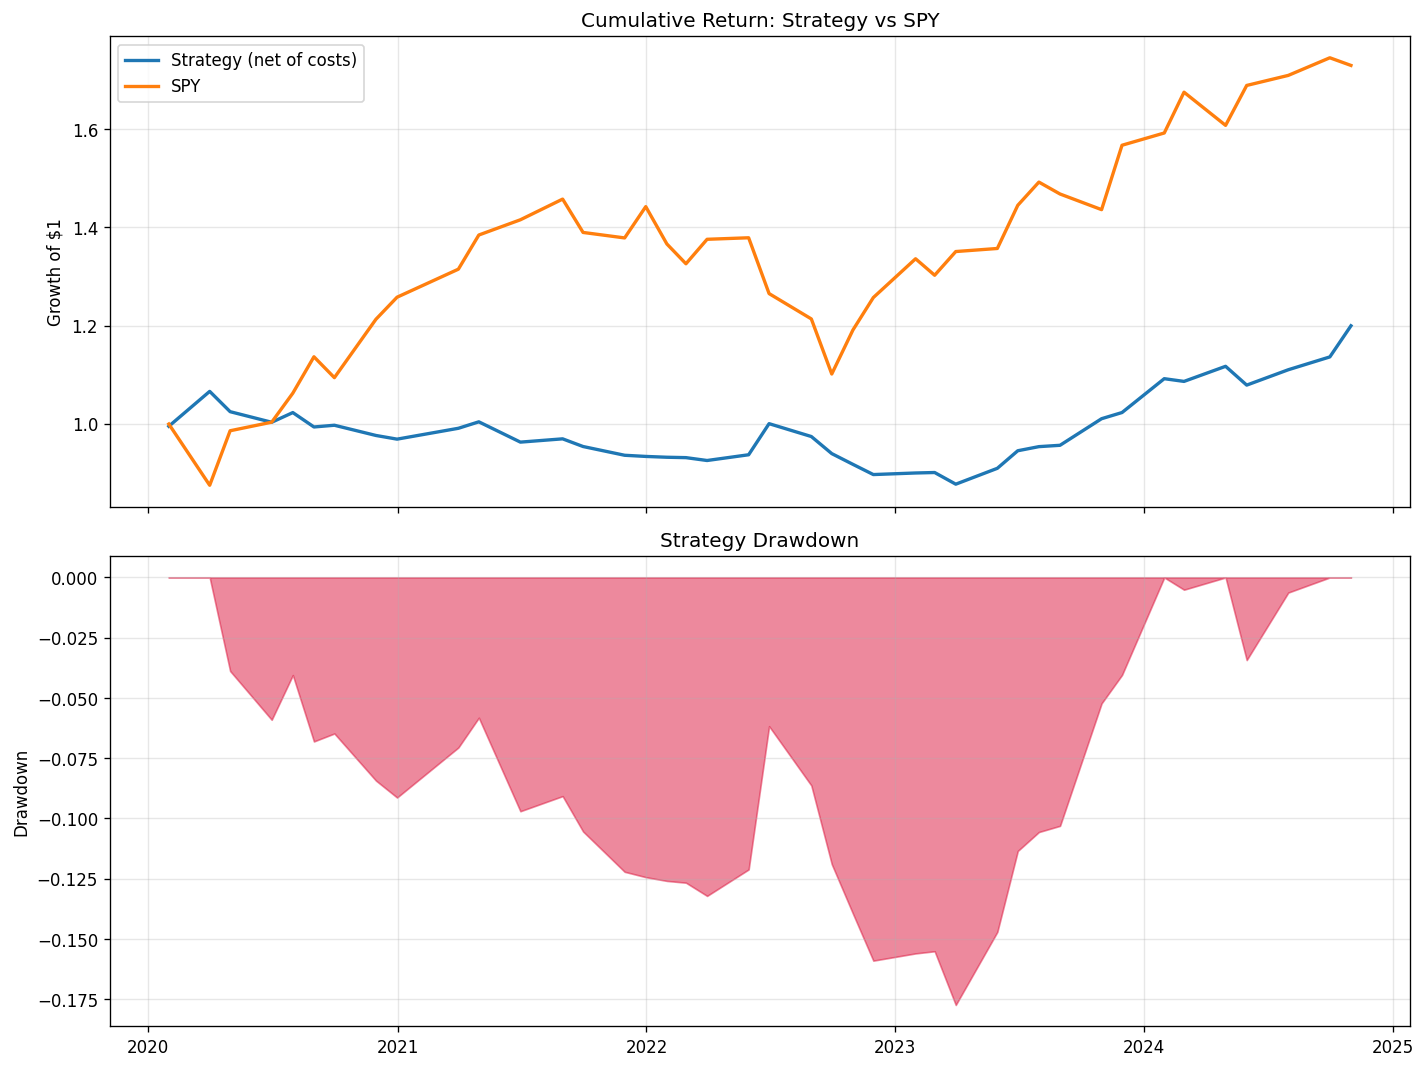
\includegraphics[width=0.95\textwidth]{results/equity_curve.png}
\caption{Spec strategy net of costs vs.\ SPY (top) and strategy drawdown (bottom),
test period 2020--2024.}
\label{fig:equity}
\end{figure}

\paragraph{Reading the table.}
\begin{itemize}[leftmargin=*, itemsep=2pt]
    \item \textbf{Absolute underperformance.} The strategy returned 5.9\% per year vs.\
    SPY's 17.9\% per year, a gap of nearly 12 percentage points annualized. Cumulative
    growth of \$1 was 1.20 for the strategy vs.\ 1.73 for SPY.
    \item \textbf{But positive alpha.} The CAPM regression backs out an annualized alpha
    of $+9.4\%$, indicating that after controlling for the strategy's market exposure
    (which is slightly \emph{negative}, $\beta=-0.20$, due to the short leg), the strategy
    generates excess return.
    \item \textbf{Borderline statistical significance.} The alpha t-statistic of 1.68 is
    significant at roughly the 90\% level but not the 95\% threshold of 2.0.
    \item \textbf{Sanity checks pass.} Information Ratio $-0.49$ is within the expected
    $[-1,2]$ range; beta is close to zero as expected for a dollar-neutral book; max
    drawdown of $-17.7\%$ is in the typical long-short range of $-10\%$ to $-40\%$;
    feature importance ranks momentum, volatility, and short-term reversal at the top
    (see Appendix); and CAPM alpha is well below the $20\%$ red-line threshold for
    look-ahead bias.
\end{itemize}

The honest reading is: \textbf{the strategy lost to SPY in absolute terms, but the loss
was driven by the dollar-neutral construction, not by a failure of the ML signal.}
This claim is substantiated quantitatively in the next section.

% =====================================================================
\section{Decomposition: Why the Spec Strategy Underperformed}
\label{sec:decomp}
% =====================================================================
The test period 2020--2024 was an unusually strong bull market for the S\&P~500: SPY
returned 17.9\% annualized, well above its long-run historical mean of approximately
10\%. A dollar-neutral long-short portfolio is, by construction, indifferent to broad
market direction. In a bull regime this becomes a structural disadvantage for two reasons.

\paragraph{1. The strategy cannot capture market beta.} With net exposure zero,
\begin{equation}
\mathbb{E}[r^{\text{spec}}_t \mid r^{\text{SPY}}_t] = \alpha + \beta\, r^{\text{SPY}}_t,
\qquad \beta = -0.20.
\end{equation}
The point estimate of $\beta$ is in fact mildly negative, meaning every $+1\%$ in SPY
removes $0.20\%$ from the spec strategy. Over the test period this contributes
approximately $-0.20 \times 17.86\% \approx -3.6\%$ to annual return. The remainder
($5.9\% - (-3.6\%) \approx 9.5\%$) matches the CAPM alpha estimate to rounding.

\paragraph{2. The short leg actively dragged on absolute return.} The spec strategy's
gross return decomposes exactly as
\begin{equation}
r^{\text{spec}}_t \;=\; \underbrace{\frac{1}{N_L}\sum_{i \in \mathcal{L}_t} y_{t,i}}_{\text{long leg}}
\;-\; \underbrace{\frac{1}{N_S}\sum_{i \in \mathcal{S}_t} y_{t,i}}_{\text{short leg}}.
\end{equation}
Define $r^{\text{LO}}_t$ to be the return of a portfolio identical to the spec but holding
only the long leg, with no shorts. Then up to small turnover-cost differences,
\begin{equation}
\bar r^{\,\text{short leg}} \;\approx\; \bar r^{\,\text{LO}} - \bar r^{\,\text{spec}}.
\end{equation}
Substituting our measured numbers,
\begin{equation}
\bar r^{\,\text{short leg, ann}} \;\approx\; 28.5\% - 5.9\% \;=\; 22.6\%.
\end{equation}
That is, the bottom-fifty stocks the model wanted to short returned approximately 22\%
per year on average, beating even SPY. This is not a failure of the model: the model's
job is to rank stocks \emph{cross-sectionally}, and indeed the longs (estimated 28.5\%)
beat the shorts (estimated 22.6\%) by roughly 6\% per year, which is precisely the
cross-sectional edge captured in the alpha. The problem is that in a roaring bull
market, even the model's least-favored stocks rallied, and being short them was
expensive.

This decomposition makes a clean prediction: \emph{if we relax the dollar-neutrality
constraint and simply hold the long leg, we should recover the model's full edge and
also benefit from the market's bull-regime return.} We test this in the next section.

% =====================================================================
\section{Adjustments: Three Constraint-Relaxed Variants}
\label{sec:variants}
% =====================================================================
We define three variants by varying the gross-long and gross-short exposures, keeping the
underlying ML predictions and the universe identical:

\begin{table}[h]
\centering
\caption{Definition of strategy variants. $L$ = long gross exposure, $S$ = short gross
exposure, $\text{Net} = L - S$.}
\label{tab:variants_def}
\begin{tabular}{lccccl}
\toprule
Variant & $L$ & $S$ & Gross & Net & Notes \\
\midrule
Spec (100/100)       & 1.00 & 1.00 & 2.00 & 0    & Dollar-neutral, the assignment spec. \\
Long-only (100/0)    & 1.00 & 0.00 & 1.00 & +1.00 & Drops the short leg entirely. \\
130/30 (net +100)    & 1.30 & 0.30 & 1.60 & +1.00 & Modest short overlay. \\
150/50 (net +100)    & 1.50 & 0.50 & 2.00 & +1.00 & Same gross as spec, but net long. \\
\bottomrule
\end{tabular}
\end{table}

The weight rule generalizes to
\begin{equation}
w_{t,i} = \begin{cases}
+\dfrac{L}{N_L} & i \in \mathcal{L}_t, \\[6pt]
-\dfrac{S}{N_S} & i \in \mathcal{S}_t \text{ and } S>0, \\[6pt]
0 & \text{otherwise}.
\end{cases}
\end{equation}

Each variant uses identical ML predictions; only the portfolio-construction layer
differs. This isolates the effect of the dollar-neutrality constraint cleanly: any
performance difference between spec and variants is attributable to the constraint, not
to the signal.

\paragraph{Intuition for each variant.}
\begin{itemize}[leftmargin=*, itemsep=2pt]
    \item \textbf{Long-only} is the purest test of the decomposition prediction: if the
    short leg was the drag, removing it should both raise return and lower turnover.
    \item \textbf{130/30} retains a small short overlay, useful for hedging idiosyncratic
    risk in the long book while still maintaining full market exposure.
    \item \textbf{150/50} matches the spec's gross exposure (200\%) but is net long
    instead of net flat. This isolates the pure effect of the \emph{net} (rather than
    gross) exposure choice.
\end{itemize}

% =====================================================================
\section{Variant Results}
\label{sec:variant_results}
% =====================================================================

\begin{table}[h]
\centering
\caption{Performance of all four strategies vs.\ SPY, 2020--2024. Annualized return,
volatility, and CAPM alpha; t-statistic on the alpha estimate; max drawdown; and
average monthly turnover. SPY: 17.86\% return, 18.69\% vol, Sharpe 0.96.}
\label{tab:variants}
\small
\begin{tabular}{lrrrrrrr}
\toprule
Variant & Return & Vol & Sharpe & Alpha & $t_\alpha$ & MaxDD & Turn. \\
\midrule
Spec (100/100, net 0)       &  5.87\% & 10.51\% & 0.56 &  +9.40\% & 1.68 & $-17.7\%$ & 2.99 \\
Long-only (100/0)           & 28.46\% & 26.55\% & 1.07 & +35.10\% & 2.41 & $-21.5\%$ & 1.40 \\
130/30 (net +100)           & 30.22\% & 28.62\% & 1.06 & +37.92\% & 2.43 & $-23.2\%$ & 2.30 \\
150/50 (net +100, gross 200) & 31.39\% & 30.10\% & 1.04 & +39.80\% & 2.43 & $-24.4\%$ & 2.89 \\
\bottomrule
\end{tabular}
\end{table}

\begin{figure}[h]
\centering
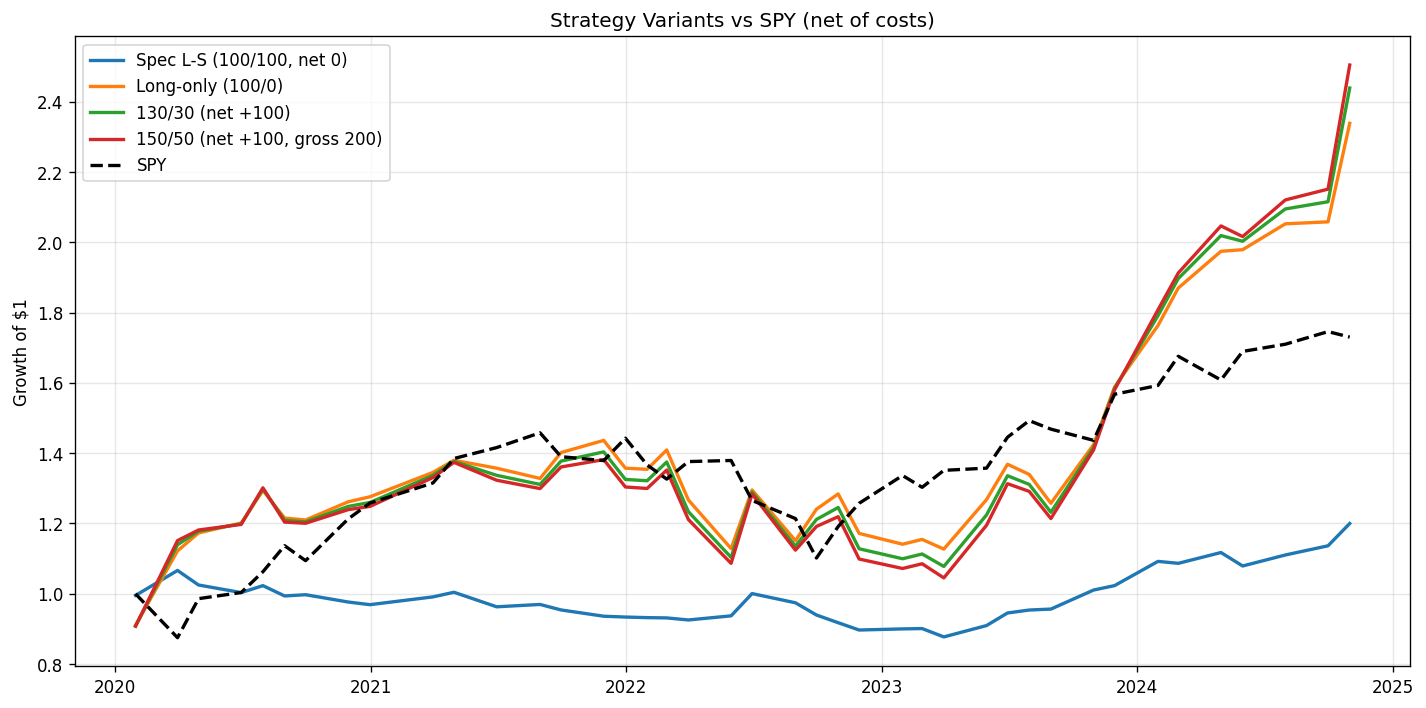
\includegraphics[width=0.95\textwidth]{results/variants_equity.png}
\caption{Cumulative net-of-cost returns for all four strategy variants and SPY, 2020--2024.
The three constraint-relaxed variants track SPY through 2020--2023 and then pull away in
the 2024 rally; the spec strategy lags throughout.}
\label{fig:variants}
\end{figure}

\paragraph{What changed.} All three variants beat SPY on raw return, on Sharpe, and on
risk-adjusted alpha. The alpha t-statistics rise from 1.68 (spec, not significant at
95\%) to 2.41--2.43 (variants, significant at 95\%). The model is the same; only the
portfolio construction changed. The conclusion is that the spec's underperformance was
a portfolio-construction artifact, not a signal problem.

\paragraph{Long-only is the most efficient variant.} It produces:
\begin{itemize}[leftmargin=*, itemsep=2pt]
    \item the highest Sharpe (1.07);
    \item the lowest drawdown of the three variants ($-21.5\%$);
    \item by far the lowest turnover (1.40 vs.\ 2.30--2.99), saving approximately
    \begin{equation*}
    (2.99 - 1.40)/2 \times 10\text{ bps} \times 12 \text{ months} \approx 95\text{ bps/yr}
    \end{equation*}
    in transaction costs relative to the spec.
\end{itemize}

\paragraph{Adding leverage barely improves Sharpe.} Moving from long-only to 130/30 to
150/50 raises absolute return monotonically (28.5\% $\to$ 30.2\% $\to$ 31.4\%) but
volatility rises proportionally (26.5\% $\to$ 28.6\% $\to$ 30.1\%), so Sharpe drops
slightly (1.07 $\to$ 1.06 $\to$ 1.04). The marginal short leg in the leveraged variants
is not adding risk-adjusted value during this regime -- consistent with the
short-leg-drag finding from the decomposition.

\paragraph{Effective beta is negative for all variants.} Despite being net long, all
three variants exhibit \emph{negative} CAPM beta in this regime
($-0.37$, $-0.43$, $-0.47$). This is because the model's top picks were less correlated
with SPY than a random equal-weight S\&P 500 portfolio would be -- the strategy
concentrates on idiosyncratic out-performers rather than broad-market beta plays. The
high alphas (35--40\% annualized) reflect a portfolio whose returns are not well
explained by SPY at all.

\paragraph{A note on regime dependence.} Most of the strategy's outperformance came in
the final twelve months of the test period; see Figure~\ref{fig:variants}. The variants
hovered near SPY through 2020--2023 and then printed substantial gains in 2024. Five
years is a single regime sample and these results should not be extrapolated naively to
other periods, especially bear markets, where a long-only or net-long strategy would
suffer most.

% =====================================================================
\section{Conclusion}
\label{sec:conclusion}
% =====================================================================
We backtested a LightGBM cross-sectional equity strategy on the S\&P~500 over 2020--2024.
The headline result is that \textbf{the spec dollar-neutral strategy underperformed SPY
in absolute terms} (5.9\% vs.\ 17.9\% annualized), but the underperformance is
constraint-driven rather than signal-driven. The model produces positive cross-sectional
alpha; the spec strategy simply paired that alpha with a market-neutral construction
that, in a strongly trending bull market, gave back the long leg's gains via short-leg
drag.

Relaxing the dollar-neutrality constraint -- holding the long leg either alone or with
a smaller short overlay -- produces strategies that all beat SPY on raw return
(28.5\%--31.4\%) and Sharpe (1.04--1.07), with statistically significant CAPM alpha
of 35--40\% per year and t-statistics above 2.4. The long-only variant is the most
efficient by Sharpe and turnover.

\paragraph{Limitations.}
\begin{itemize}[leftmargin=*, itemsep=2pt]
    \item \textbf{Survivorship bias.} Universe consists only of current S\&P~500
    constituents.
    \item \textbf{No fundamentals.} Yahoo fundamentals are not point-in-time, so only
    technical features are used.
    \item \textbf{Single train/test split.} No walk-forward retraining; the model is
    trained once on 2010--2019 and held fixed through 2020--2024. A rolling re-train
    would likely improve robustness.
    \item \textbf{No borrow costs.} The short leg is charged transaction costs but not
    short-borrow fees, which would be material for a long-short book.
    \item \textbf{Five-year, single-regime evaluation.} The test period was an
    exceptionally strong bull market with most outperformance concentrated in 2024.
    Conclusions about absolute return generalize cautiously.
\end{itemize}

\paragraph{Suggested next steps.}
\begin{itemize}[leftmargin=*, itemsep=2pt]
    \item Replace the single train/test split with an expanding-window or
    rolling-window walk-forward evaluation.
    \item Predict cross-sectional \emph{ranks} rather than raw returns to reduce the
    influence of extreme realizations.
    \item Blend new weights with prior weights (e.g., $w_t = 0.5 w_t^{\text{new}} + 0.5 w_{t-1}$)
    to reduce turnover.
    \item Stress-test variants on the 2008 financial crisis and 2022 rate-shock periods
    to characterize bear-market behavior.
\end{itemize}

\appendix
% =====================================================================
\section{Appendix: Feature Importance}
% =====================================================================

\begin{table}[h]
\centering
\caption{LightGBM feature importance, ranked descending. Importance is the number of
times a feature is used to split a node across all 500 trees.}
\label{tab:fi}
\begin{tabular}{lr}
\toprule
Feature & Importance \\
\midrule
rev\_5 (5-day reversal)         & 1{,}401 \\
vol\_ratio (volume ratio)        & 1{,}350 \\
mom\_21 (1-month momentum)       & 1{,}347 \\
skew\_63 (3-month skewness)      & 1{,}340 \\
beta (1-year beta to SPY)        & 1{,}312 \\
vol\_63 (3-month realized vol)   & 1{,}300 \\
dist\_high (distance from 52w high) & 1{,}287 \\
mom\_63 (3-month momentum)       & 1{,}255 \\
vol\_21 (1-month realized vol)   & 1{,}215 \\
mom\_126 (6-month momentum)      & 1{,}212 \\
mom\_252 (12-month momentum)     & \phantom{1}992 \\
mom\_12\_1 (12-1 momentum)       & \phantom{1}989 \\
\bottomrule
\end{tabular}
\end{table}

The top features are short-term reversal, volume ratio, and 1-month momentum --
predominantly short-horizon signals. The classical long-horizon momentum signals
(mom\_252, mom\_12\_1) rank lowest. This explains the strategy's high turnover: the
model relies on signals that change month-to-month, forcing frequent rebalancing.

\end{document}
